\documentclass{article}

% Boilerplate {{{

\usepackage{amsmath}
\usepackage{unicode-math}
\setmainfont{XITS}
\setmathfont{XITS Math}
\usepackage{tikz}
\usetikzlibrary{matrix}
\usepackage{newunicodechar}
\usepackage{galois}
\usepackage{amsthm}

\theoremstyle{definition}
\newtheorem*{definition}{Definition}
\newtheorem*{example}{Example}

\theoremstyle{plain}
\newtheorem*{lemma}{Lemma}
\newtheorem{theorem}{Theorem}
\newtheorem{corrolary}{Corrolary}

\newcommand{\iif}{\underline{\text{if}}}
\newcommand{\case}{\underline{\text{case}}}
\newcommand{\halt}{\underline{\text{halt}}}
\newcommand{\lam}{\underline{\text{λ}}}
\newcommand{\add}{\text{add1}}
\newcommand{\sub}{\text{sub1}}
\newcommand{\gez}{\text{gez}}
\newcommand{\INT}{\text{INT}}
\newcommand{\TRUE}{\text{TRUE}}
\newcommand{\FALSE}{\text{FALSE}}
\newcommand{\ddo}{\operatorname{do}}
\newcommand{\llet}{\operatorname{let}}
\newcommand{\return}{\operatorname{return}}
\newcommand{\getstore}{\operatorname{get-σ}}
\newcommand{\putstore}{\operatorname{put-σ}}
\newcommand{\getenv}{\operatorname{get-ρ}}
\newcommand{\putenv}{\operatorname{put-ρ}}
\newcommand{\gettime}{\operatorname{get-τ}}
\newcommand{\puttime}{\operatorname{put-τ}}
\newcommand{\coercebool}{\operatorname{↓𝔹}}
\newcommand{\coercekon}{\operatorname{↓λ₁}}
\newcommand{\coercefun}{\operatorname{↓λ₂}}
\newcommand{\liftpowerset}{\operatorname{↑𝒫}}
\newcommand{\touchedcall}{\operatorname{𝓉𝒞}}
\newcommand{\touchedvar}{\operatorname{𝓉Var}}

\newcommand{\C}{L}
\newcommand{\A}{\widehat{L}}

\newcommand{\Csteps}{↦}
\newcommand{\Asteps}{\ \widehat{↦}\ }

\newcommand{\Ce}{e}
\newcommand{\Ae}{\widehat{e}}

\newcommand{\AStore}{\widehat{Store}}
\newcommand{\AEnv}{\widehat{Env}}
\newcommand{\ATime}{\widehat{Time}}
\newcommand{\AVal}{\widehat{Val}}

\newcommand{\PM}{𝒫\ }
\newcommand{\PT}{𝒫_T\ }

\newcommand{\SM}{State}
\newcommand{\ST}{State_T}

\newenvironment{donotbreak}
{\\[0.5\baselineskip]\begin{minipage}{\linewidth}}
{\end{minipage}\\[0.5\baselineskip]}

% \usepackage{multicol}

% \newunicodechar{λ}{\lambda}
% \newunicodechar{→}{\rightarrow}
% \newunicodechar{𝒯}{\mathcal{T}}
% \newunicodechar{∀}{\forall}
% \newunicodechar{∘}{\circ}
% \newunicodechar{𝒫}{𝒫\ }


% \usepackage{amssymb}
% \usepackage{listings}
% \usepackage{stmaryrd}
% \usepackage{wasysym}
% \usepackage{cite}
% \usepackage{pgfplots}
% \usepackage{minted}
% \usepackage{float}
% \usepackage{caption}
% \usepackage{fontspec}
% \setmonofont{Inconsolata}
% % \usepackage{hyperref}
% 
% \lstset{basicstyle=\footnotesize\ttfamily,language=haskell}
% \lstMakeShortInline|
% 
% \newmintedfile[haskell]{haskell}{}
% \newmintinline[h]{haskell}{}
% \newmintinline[p]{text}{}
% 
% \newenvironment{itemizenobreak}
% {\\[0.5\baselineskip]\begin{minipage}{\linewidth}\begin{itemize}}
% {\end{itemize}\end{minipage}\\[0.5\baselineskip]}
% 
% 
% \newcommand{\DSS}{\text{\lstinline|SS|}}
% \newcommand{\DSSAbs}{\widehat{\text{\lstinline|SS|}}}
% \newcommand{\Dstep}{\text{\lstinline|step|}}
% \newcommand{\DstepAbs}{\widehat{\text{\lstinline|step|}}}
% 
% %%% pulled from internet (stack overflow user Christian Feuersänger) %%%
% % argument #1: any options
% \newenvironment{customlegend}[1][]{%
%     \begingroup
%     % inits/clears the lists (which might be populated from previous
%     % axes):
%     \csname pgfplots@init@cleared@structures\endcsname
%     \pgfplotsset{#1}%
% }{%
%     % draws the legend:
%     \csname pgfplots@createlegend\endcsname
%     \endgroup
% }%
% 
% % makes \addlegendimage available (typically only available within an
% % axis environment):
% \def\addlegendimage{\csname pgfplots@addlegendimage\endcsname}
% 


\title{Abstract Control in Static Analysis}
\author{David Darais}
\date{\today}

\begin{document}
\maketitle

% }}}

% Abstract {{{
\begin{abstract}
\end{abstract}
% }}}

\tableofcontents

% Introduction {{{
\section{Introduction}
\label{section:Introduction}

% A static analysis has two components: 
% \begin{itemize}
% \item A \emph{computation} which computes some set of facts about the execution of a program.
% \item A \emph{proof of correctness} about the computation.
% \end{itemize}
% 
% We are motivated by static analysis techniques which are:
% \begin{itemize}
% \item Compartmental: Various aspects of the analysis have been separated from each other and are understood in isolation.
% \item Modular: Design choices in one aspect of the analysis do not restrict design choices of another.  
%       This property is important for both computational and correctness components of an analysis.
% \item Language Agnostic: A given analysis technique can be seamlessly transfered from one semantics to another.
% \item Correct: The proof of correctness should exist, and there should be a framework for establishing it.
% \item Derived: Either the computational artifact or the correctness proof should be obtained "for free" from the other.
% \end{itemize}
% 
% Our framework compartmentalizes:
% \begin{itemize}
% \item Abstract domain a la Cousot.
% \item Abstract time and address a la Van Horn and Might.
% \item Intensional optimizations a la Van Horn and Might. 
% \item Object-sensitivity a la Smaragdakis.
% \item Analysis control properties.
% \end{itemize}
% 
% Our framework is:
% \begin{itemize}
% \item Compartmental: Each of the above concerns are separated and independent.
% \item Modular: Design choices in one axis is completely independent of others
% \item Language Agnostic: All axis other than abstract domain are fully language agnostic.
% \item Correct: A correctness framework is described and each axis is proven correct in isolation.
% \item Derived: The correctness of an analysis using our framework comes for free.
% \end{itemize}
% 
% Analysis control properties are the primary topic of this work.
% We merely note that the other axis in the design space are implemented in our framework using existing techniques.
% 
% Contributions:
% \begin{itemize}
% \item Computational artifacts and correctness proofs for the axis of abstract control, which captures the choice of flow and path sensitivity.
% \item Computational artifacts and correctness proofs for intensional optimizations (gargabe collection and mcfa) independent of abstract control.
% \item Language independent proofs of refinement for flow-sensitivity and path-sensitivity choices using the monadic abstraction.
% \end{itemize}
 
% }}}

% Background {{{
\section{Background}
\label{section:Background}
 
% Notation {{{
\subsection{Notation}
\label{section:Background:Notation}

We use traditional notation for function definitions and applications rather than lambda calculus notation.
For example, we will write:
\begin{equation*}
compose(g, f, x) ≔ g(f(x))
\end{equation*}
rather than:
\begin{equation*}
compose\; g\; f\; x ≔ g\; (f\; x)
\end{equation*}

We use lambda notation for anonymous functions.
For example, the anonymous composition function is written:
\begin{equation*}
λ(g, f, x) → g(f(x))
\end{equation*}

% }}}

% Monads {{{
\subsection{Monads}
\label{section:Background:Monads}

A basic familiarity with the concept of monads will be necessary for understanding this paper.
Some find it useful to review the concept of functor before learning about monads. 
We adopt this approach for our brief explanation of monads.

A type $(F : Set → Set)$ is called a \emph{functor} if one can:
\begin{itemize}
\item Define $map : ∀ (A, B : Set), (A → B) → (F(A) → F(B))$
\item Prove $map(id) = id$, where $id$ is the identity function $(λ(x) → x)$
\item Prove $map (g ∘ f) = map(g) ∘ map(f)$
\end{itemize}

\paragraph{Example:} 
Lists are functors, where $map$ is defined:
\begin{align*}
    map(f)(xs) ≔ &\case(xs):           \\
          Nil    &→ Nil                \\
         x ∷ xs' &→ f(x) ∷ map(f)(xs') \\
\end{align*}

\paragraph{Example:} $map(isEven)([1, 2, 3, 4]) = [False, True, False, True]$

Likewise a type $(ℳ  : Set → Set)$ is called a \emph{monad} if one can:
\begin{itemize}
\item Define $extend : ∀ (A, B : Set), (A → ℳ (B)) → (ℳ (A) → ℳ (B))$
\item Prove unit and associativity laws (not mentioned here).
\end{itemize}
The only difference from the definition of functor is in the the first argument.
For monads, this argument is allowed to be a \emph{monadic} $(A → ℳ (B))$, rather than a pure function $(A → B)$.

\paragraph{Example:} Lists are monads, where $extend$ is defined:
\begin{align*}
    extend(f)(xs) ≔ &\case(xs):              \\
                Nil &→ Nil                   \\
            x ∷ xs' &→ f(x) ⧺ extend(f)(xs') \\
\end{align*}

\paragraph{Example:} 
$extend(λ(x) → [x + 1, x - 1])([10, 100]) = [9, 11, 99, 101]$

$extend$ for lists can also be understood as $concat$ followed by $map$:
\paragraph{Example:} 
\begin{align*}
extend(f)([10, 100]) &= concat(map(f)([10, 100]))    \\
                     &= concat([[9, 11], [99, 101]]) \\
                     &= [9, 11, 99, 101]             \\
\end{align*}
For all monads, it is equivalent to define $return$, $map$ and $join$, where:
\begin{equation*}
join : ∀ (A : Set), ℳ (ℳ (A)) → ℳ (A)
\end{equation*}
As we have just seen, $join$ for the list monad is just $concat$.

% }}}

% Monad Transformers {{{
\subsection{Monad Transformers}
\label{section:Background:MonadTransformers}

Monad transformers are functions between monads.
Where a monad $ℳ $ will have type $Set → Set$, a monad transformer $𝒯$ will have type $(Set → Set) → (Set → Set)$.

Monad transformers are used to extend an existing monad to support another effect.
The three monads used in this work are the state monad, powerset monad, and the identity monad.
The state monad is notated $\SM(𝓈)$ (carrying a single cell of type $𝓈$), the powerset monad is notated $\PM$, and the identity is notated $ID$.
The state and powerset monad transformer equivalents are notated $\ST(𝓈)(ℳ )$ and $\PT(ℳ )$ where $ℳ $ is the underlying monad.
The state monad has $get$ and $put$ effects, whereas the powerset monad has a $nondeterminism$ effect.
The transformer versions of both of these monads allow you to combine effects piecewise.

\paragraph{Example:}
$\ST(ℤ)(\PT(ID))$ is a monad which has $get$ and $put$ effects for a single cell of integer state, in addition to nondeterminism effects.

The definitions, details and proofs of all monads used in our work are given in section \ref{section:Proofs}.

% }}}

% Small Step Semantics {{{
\subsection{Small-Step Semantics}
\label{section:Background:SmallStepSemantics}

This work follows the small-step operational approach to language semantics pioneered by Plotkin and Felleisen.
In small-step operational semantics, the meaning of an expression $e$ of a language is given by the transitive closure of some step relation $e ↦ e'$.
This yields a state-machine approach to semantics.
Exploring the meaning of $e$ reduces to exploring all possible transitions reachable from $e$ through $↦$.
This contrasts to previously developed deontational approaches, where the meaning of $e$ must be given all at once by a denotation function $⟦ e ⟧$.
This denotation function can quickly demand lots of mathematical machinery.
Small-step operational methods side-step the need for such machinery.

The small-step operation framework supports arbitrary step relations $e ↦ e'$.  
However for our purposes $↦$ will be always be a function-like form of \emph{decidable} relation, i.e. a multifunction.

% }}}

% Abstract Interpretation {{{
\subsection{Abstract Interpretation}
\label{section:Background:AbstractInterpretation}

Abstract Iterpretation (AI) is a formal framework for program analysis pioneered by Cousot and Cousot.
In the setting of abstract interpretation, a program analysis is just an alternate semantics over an abstract domain.
To distinguish the original semantics from the alternate semantics we call the original semantics the \emph{concrete} semantics.
The alternate semantics is called the \emph{abstract} semantics\footnote{
  This terminology quickly becomes confusing because we will eventually construct an abstract machine for both semantics.
  This yields a concrete abstract machine and an abstract abstract machine. 
  This linguistic pun is exploited mercilessly in the work of Might and Van Horn as they “abstract” abstract abstract machines, yielding abstract abstract abstract machines.
}.

Consider a concrete language $\C$ and a program in that language $(\Ce : \C)$.
In the AI framework, an analysis for $\Ce$ is:
\begin{itemize}
\item 
  An abstract language $\A$.
\item 
  A relationship between $\C$ and $\A$ that defines when some $(\Ce' : \C)$ and $(\Ae' : \A)$ are related.
  This often takes the form of projecting $\A$ to $\PM(\C)$ and using the subset relation.
\item 
  An abstract version of our concrete program $\Ce$: $(\Ae : \A)$.
\item 
  An abstract version of the $\Csteps$ relation: $(\Asteps : \A × \A → Prop)$
\item 
  A method to explore every state reachable by $\Ae$ under $\Asteps$.
  This often requires $\A$ to be finite.
\end{itemize}
By convention, we put hats ($\widehat{\;\;}$) on things to name their abstract cousins.
The overall approach is summarized in the following picture:
\begin{donotbreak}\begin{center}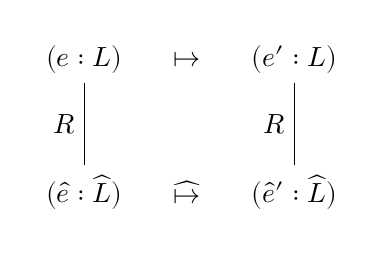
\begin{tikzpicture}[ampersand replacement=\&]

\matrix (m) [matrix of math nodes,row sep=3em,column sep=4em,minimum width=2em]
{ (\Ce : \C) \& (\Ce' : \C) \\
  (\Ae : \A) \& (\Ae' : \A) \\
} ;
\path

(m-1-1) 
edge [white]
node [black] {$\Csteps$} 
(m-1-2)

(m-2-1) 
edge [white]
node [black] {$\Asteps$}
(m-2-2)

(m-1-1) 
edge
node [left] {$R$} 
(m-2-1)

(m-1-2) 
edge
node [left] {$R$} 
(m-2-2)

;

\end{tikzpicture}\end{center}\end{donotbreak}

This picture takes place at some point in the analysis process.
$\Ce$ is the current program (possibly the result of running the base program for a little while).
$\Ae$ is a valid abstraction of $\Ce$, where this validity is expressed some relation $R$ holding between $\Ce$ and $\Ae$.
$\Ce'$ is some next state of execution of $\Ce$, and likewise for $\Ae$/$\Ae'$.
In order to be a correct analysis, it must be guaranteed that $\Ce'$ and $\Ae'$ will be related.
The logical structure of the picture, which states the correctness of the analysis, is given by:
\begin{equation*}
∀ (\Ce,\Ce' : \C ) (\Ae,\Ae' : \A), (\Ce R \Ae) ∧ (\Ce \Csteps \Ce') ∧ (\Ae \Asteps \Ae') ⇒  (\Ce' R \Ae')
\end{equation*}

% }}}

% Galois Connections {{{
\subsection{Galois Connections}
\label{section:Background:GaloisConnections}

The AI setting can be elegently simplified and enriched through the use of \emph{galois connections}.
Galois connections serve as a unifying framework for establishing the “relationship between $\C $ and $\A$” mentioned in the previous section.

A galois connection between two posets (sets with a partial order) $\C$ and $\A$ is notated $\C\galois{α}{γ}\A$ and contains:
\begin{itemize}
\item $(α : \C → \A)$ where $α$ is monotonic
\item $(γ : \A → \C )$ where $γ$ is monotonic
\item A proof that $(γ ∘ α)$ is expansive: $∀ (x : \C ), x ⊑ γ(α(x))$
\item A proof that $(α ∘ γ)$ is contractive: $∀ (y : \A), α(γ(y)) ⊑ y$
\end{itemize}
The last two properties can be succinctly stated as $(α ∘ γ ⊑ id ⊑ γ ∘ α)$\footnote{
  This uses the logical monotonicity relation $f ⊑ g ⇔  (x ⊑ y ⇒  f(x) ⊑ g(y))$ for the function space.
}.
Equivalent to all four properties is the property $x ⊑ γ(y) ⇔  α(x) ⊑ y$.

\paragraph{Example:}
Given a galois connection $\C\galois{α}{γ}\A$, there exists a galois connection $(\C → \C)\galois{α'}{γ'}(\A → \A)$ where:
\begin{align*}
α'(f : \C → \C) &≔ α ∘ f ∘ γ \\
γ'(g : \A → \A) &≔ γ ∘ g ∘ α \\
\end{align*}

\paragraph{Example:} 
The language $(\PM(ℤ),+,*)$ forms a galois connection with the language $(\PM(\{ EVEN, ODD \}),∧,∨)$ where:
\begin{align*}
α(zs : \PM(ℤ))               &≔ ⋃ \{ \{ EVEN  \;|\; ∃ z ∈ zs ∧ Even(z) \},  \{ ODD   \;|\; ∃ z ∈ zs ∧ Odd(z) \} \} \\
γ(ts : \PM(\{ EVEN, ODD \})) &≔ ⋃ \{ \{ z ∈ ℤ \;|\; EVEN ∈ ts ∧ Even(z) \}, \{ z ∈ ℤ \;|\; ODD ∈ ts ∧ Odd(z) \} \} \\
\end{align*}

Galois connections simplify the AI framework by using $x ⊑ γ(y)$ or (equivalently) $α(x) ⊑ y$ as the relation $(x R y)$.
Galois connections are a natural and general way of placing partial orders \emph{on sets themselves}.
$x ⊑ γ(y)$ can be seen as a heterogenous extension of $x ⊑ y$ when $(x : A)$ and $(y : B)$ live in different sets. 
This heterogenous order is given meaning when there exists a galois connection $A\galois{α}{γ}B$.
One can also think of galois connections as something like an isomorphism, but with a weaker round-trip property.
(An isomorphism would require $α ∘ γ = id = γ ∘ α$.)

Using galois connections, the AI framework introduced in the previous section can be re-stated. In the AI framework, an analysis for $\Ce$ is:
\begin{itemize}
\item 
  An abstract language $\A$.
\item 
  A galois connection $\C\galois{α}{γ}\A$.
\item 
  An abstract version of the $\Csteps$ relation: $(\Asteps : \A × \A → Prop)$
\item 
  A way to explore every state reachable by $\Ae$ under $\Asteps$.
  This often requires $\A$ to be finite.
\end{itemize}
The overall approach is summarized in the following picture:
\begin{donotbreak}
\begin{center}
\begin{tabular*}{0.66\textwidth}{@{\extracolsep{\fill}} c c}

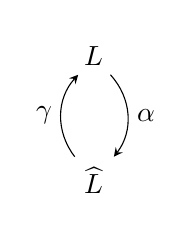
\begin{tikzpicture}[ampersand replacement=\&]
\matrix (m) [matrix of math nodes,row sep=3em,column sep=4em,minimum width=2em]
{ \C \\
  \A \\
} ;
\path [-stealth]

(m-1-1) 
edge [bend left=40]
node [right] {$α$} 
(m-2-1)

(m-2-1) 
edge [bend left=40]
node [left] {$γ$} 
(m-1-1)

;
\end{tikzpicture}

&

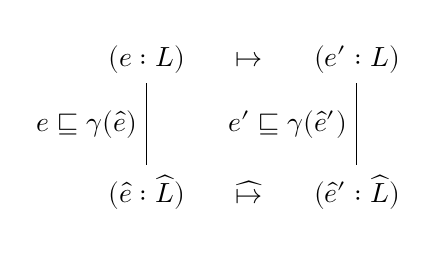
\begin{tikzpicture}[ampersand replacement=\&]
\matrix (m) [matrix of math nodes,row sep=3em,column sep=4em,minimum width=2em]
{ (\Ce : \C) \& (\Ce' : \C) \\
  (\Ae : \A) \& (\Ae' : \A) \\
} ;
\path

(m-1-1) 
edge [white]
node [black] {$\Csteps$} 
(m-1-2)

(m-2-1) 
edge [white]
node [black] {$\Asteps$}
(m-2-2)

(m-1-1) 
edge
node [left] {$\Ce ⊑ γ(\Ae)$} 
(m-2-1)

(m-1-2) 
edge
node [left] {$\Ce' ⊑ γ(\Ae')$} 
(m-2-2)

;
\end{tikzpicture}

\end{tabular*}
\end{center}
\end{donotbreak}

As before, the logical structure of the picture is given by:
\begin{equation*}
∀ (\Ce,\Ce' : \C ) (\Ae,\Ae' : \A), (\Ce ⊑ γ(\Ae)) ∧ (\Ce \Csteps \Ce') ∧ (\Ae \Asteps \Ae') ⇒  (\Ce' ⊑ γ(\Ae'))
\end{equation*}
The statement of this property can be simplified further as $\Csteps ⊑ γ(\Asteps)$.
This uses the definition of galois connections for function spaces shown in a previous example.

Using a galois connection $\C\galois{α}{γ}\A$ and abstract step function $\Asteps ⊑ γ(\Csteps)$, the analysis process becomes more specific:
\begin{itemize}
\item Translate $(\Ce : \C)$ to $(α(\Ce) : \A)$
\item Explore all abstract states $\Ae'$ states reachable from $α(\Ce)$.
\item All reachable concrete states are summarized by projecting each $γ(\Ae')$ back to $\C$.
\end{itemize}

The galois connection framework simultaneously guarantees the \emph{soundness} and \emph{tightness} of this method.
Soundness tells us that if we abstract, take an abstract step, and then concretize, that the result is an approximation of taking a concrete step.
Soundness tells us that we can trust the results of the analysis.
\begin{donotbreak}
\begin{center}

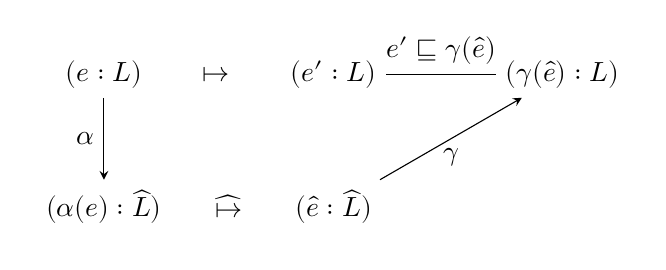
\begin{tikzpicture}[ampersand replacement=\&]
\matrix (m) [matrix of math nodes,row sep=3em,column sep=4em,minimum width=2em]
{ (\Ce : \C)    \& (\Ce' : \C) \& (γ(\Ae) : \C) \\
  (α(\Ce) : \A) \& (\Ae : \A)  \&               \\
} ;
\path [-stealth]

(m-1-1) 
edge
node [left] {$α$} 
(m-2-1)

(m-2-1) 
edge [white]
node [black] {$\Asteps$}
(m-2-2)

(m-2-2)
edge
node [below] {$γ$} 
(m-1-3) 

(m-1-1) 
edge [white]
node [black] {$\Csteps$} 
(m-1-2)

;

\path

(m-1-2)
edge
node [above] {$\Ce' ⊑ γ(\Ae)$}
(m-1-3)

;
\end{tikzpicture}

\end{center}
\end{donotbreak}


Tightness tells us that if we concretize, take a concrete step, and then abstract, then the result must be just as precise as taking an abstract step.
Tightness tells us that our abstract step function isn't losing precision unnecessarily, and that our abstract step $\Asteps$ is provably as strong as possible.
\begin{donotbreak}
\begin{center}

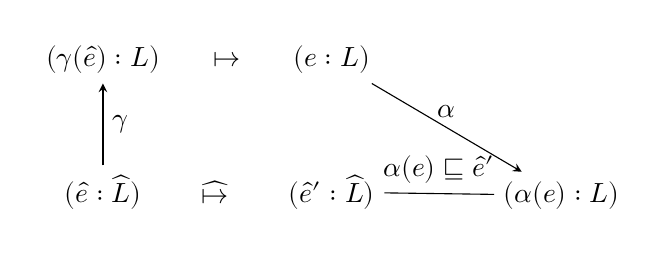
\begin{tikzpicture}[ampersand replacement=\&]
\matrix (m) [matrix of math nodes,row sep=3em,column sep=4em,minimum width=2em]
{ (γ(\Ae) : \C) \& (\Ce : \C) \&                \\
  (\Ae : \A)    \& (\Ae' : \A) \& (α(\Ce) : \C) \\
} ;
\path [-stealth]

(m-2-1) 
edge
node [right] {$γ$} 
(m-1-1)

(m-1-1) 
edge [white]
node [black] {$\Csteps$}
(m-1-2)

(m-1-2)
edge
node [above] {$α$} 
(m-2-3) 

(m-2-1) 
edge [white]
node [black] {$\Asteps$} 
(m-2-2)

;

\path

(m-2-2)
edge
node [above] {$α(\Ce) ⊑ \Ae'$}
(m-2-3)

;
\end{tikzpicture}

\end{center}
\end{donotbreak}




% }}}

% CPS {{{
\subsection{Continuation Passing Style}
\label{section:Background:ContinuationPassingStyle}

We use CPS-IF as an example language to demonstrate the benefits of our framework.
CPS is a syntactically restricted version of the lambda calculus.
CPS-IF is an extension of CPS with conditionals.
We choose CPS because the state machine for the semantics of CPS requires no call stack.
We add conditionals to make things slightly more interesting.

We define the CPS-IF language as follows:
\begin{align*}
x,y,k : Var  &⩴ ...variables...                                          \\
b,i,l : Lit  &⩴ ℤ ∪ 𝔹                                                    \\
  f,g : Lam  &⩴ \lam(x) → e \;|\; \lam(x,k) → e                          \\
    a : Atom &⩴ x \;|\; l \;|\; f \;|\; op(a)                            \\
   op : Op   &⩴ \add \;|\; \sub \;|\; \gez                               \\
    e : Exp  &⩴ \iif(a)\{e\}\{e\} \;|\; a(a) \;|\; a(a,a) \;|\; \halt(a) \\
\end{align*}



CPS-IF supports integer and boolean literals, addition and subtraction by 1, and testing if an integer is greater than or equal to zero.
The essence of CPS is in the syntactic restriction on application forms $a(a)$ and $a(a,a)$.  
Because $a$ cannot be a nested call expression, evaluating a $Call$ requires no evaluation stack.

All lambda calculus terms can be translated to CPS terms through CPS-conversion.
However, because lambda calculus terms are much easier to read, we will use lambda calculus terms for examples.
We display the CPS-converted version of examples where appropriate.

% }}}

% Control Flow Analysis {{{
\subsection{Control Flow Analysis}
\label{section:Background:ControlFlowAnalysis}

Control flow analysis is a class of analysis which is particularly important for higher-order languages.
In non-higher-order languages, it is useful to distinguish control-flow from data-flow.
The control flow of the program is a graph of what functions are called from where.
The data flow of a program is a mapping of which values can flow to which variables.
Traditionally one performs a control-flow analysis first, to find out which functions are called, and a data-flow analysis second, using the results of the control flow analysis.

In higher-order languages, data-flow and control-flow are tightly coupled.
Before you can tell which functions will be called, you need to know how values flow, because functions are themselves values.

We note that the distinction between “higher-order” languages and “non-higher-order” languages is a red herring.
Functions can be passed as values in C using function pointers, and object-oriented languages enjoy a similar circularity between control- and data- flow due to method dispatch.
You can read these statements as saying “all languages are higher order, and thus all languages need higher order control flow analysis”.
Or you can read them as saying “all languages are higher order, and we've done just fine without higher oder control flow analysis so far”.
The real distinction is in the code that you end up analysing.

We build on the tradition of control flow analysis (CFA) pioneered by Shivers, as well as recent refinements of CFA developed by Might and Van Horn.
In this tradition, the result of a control flow analysis is closer to what one would think of as a data-flow analysis, only the process accounts for higher order flow.
0CFA, the most basic control flow analysis, merely computes the set of values which might flow to a particular variable.
kCFA is a suite of context sensitive extensions to 0CFA for which functions are analyzed separately for each possible calling context.
We use 0CFA as the example analysis in this paper.
However our framework, and our implementation of it, scale to the full range of context sensitive control flow analyses.

% }}}

% }}}

% Monadic AAM {{{

\section{Monadic AAM}
\label{section:MonadicAAM}

Monadic abstract interpretation[Sergey et al. PLDI 2013] demonstrated that abstract interpreters can be built modularly using a monadic abstraction.
We build directly on this work at the level of intuition—monads serve as our pivot-point for achieving modularity.
However, in our pursuit of a modular correctness framework, our approach deviates greatly from prior work in the specific interfaces used.

First we demonstrate a simple 0CFA analysis on CPS-IF which doesn't use our framework.
The CPS-IF language is introduced in section \ref{section:Background:ContinuationPassingStyle}.
We repeat the definition here for convenience.
\begin{align*}
x,y,k : Var  &⩴ ...variables...                                          \\
b,i,l : Lit  &⩴ ℤ ∪ 𝔹                                                    \\
  f,g : Lam  &⩴ \lam(x) → e \;|\; \lam(x,k) → e                          \\
    a : Atom &⩴ x \;|\; l \;|\; f \;|\; op(a)                            \\
   op : Op   &⩴ \add \;|\; \sub \;|\; \gez                               \\
    e : Exp  &⩴ \iif(a)\{e\}\{e\} \;|\; a(a) \;|\; a(a,a) \;|\; \halt(a) \\
\end{align*}



Our abstract semantics of 0CFA will track literals (including lambdas) that appear in the program text.
For integers that do not appear in the program text, the analysis uses a single token $INT$ which conservatively approximates any possible integer.
Formally, the state space $Σ$ for the abstract machine of the abstract semantics is defined as:
\begin{align*}
v : \AVal   &⩴ \INT \;|\; l \;|\; \lam(x) → c \;|\; \lam(x,k) → c \\
σ : \AStore &≔ Var → \PM(\AVal)                                   \\
Σ           &≔ \PM(Call × \AStore)                                \\
\end{align*}
Because there are a finite many literals in the program text, we can claim there are a finite number of possible abstract values.

The abstract semantics for $Σ$ comes in two parts.  
First we define a \emph{denotation function} $𝒜 $ for $Atom$ expressions.
\begin{align*}
𝒜                            &: \AStore × Atom → \PM(\AVal) \\
𝒜 (σ,x)                      &≔ σ(x)                        \\
𝒜 (σ,l)                      &≔ \{ l \}                     \\
𝒜 (σ,\add a) | 𝒜 (σ,a) ⊑ INT &≔ \{ \INT \}                  \\
𝒜 (σ,\sub a) | 𝒜 (σ,a) ⊑ INT &≔ \{ \INT \}                  \\
𝒜 (σ,\gez a) | 𝒜 (σ,a) ⊑ INT &≔ \{ \TRUE , \FALSE \}        \\
𝒜 (σ,\lam(x) → c)            &≔ \{ \lam(x) → c \}           \\
𝒜 (σ,\lam(x)(k) → c)         &≔ \{ \lam(x)(k) → c \}        \\
\end{align*}

Second we define a \emph{step relation} (as a function) $𝒞$ for $Call$ expressions.
\begin{align*}
𝒞                        : &Call × \AStore → \PM(Call × \AStore)                                              \\
𝒞(\iif(a)\{c₁\}\{c₂\},σ) ≔ &\{ (c,σ)                                                                          \\
                           &|\; c ∈ ⋃ \{ \{ c₁ \;|\; \TRUE ∈ 𝒜 (σ,a) \}, \{ c₂ \;|\; \FALSE ∈ 𝒜 (σ,a) \} \} \\
                           &\}                                                                                \\
𝒞(a₁(a₂,a₃),σ)           ≔ &\{ (c,σ')                                                                         \\
                           &|\; (\lam(x)(k) → c) ∈ 𝒜 (σ,a₁)                                                   \\
                           &|\;             v₂ ∈ 𝒜 (σ,a₂)                                                     \\
                           &|\;             v₃ ∈ 𝒜 (σ,a₃)                                                     \\
                           &|\;             σ' ≔ σ ⊔ [x ↦ v₂] ⊔ [k ↦ v₃]                                      \\
                           &\}                                                                                \\
𝒞(\halt(a),σ)            ≔ &\{ (\halt(a),σ) \}                                                                \\
\end{align*}
(We omit the $(a₁(a₂))$ case. It is directly analogous to $(a₁(a₂,a₃))$).

The complete analysis of a program $c$ is defined as the least fixed point of a \emph{collection semantics} for the relation $𝒞$:
\begin{align*}
\text{analysis} ≔ μ(Σ) → \{(c,⊥)\} ⊔ 𝒞^{⋆}(Σ)
\end{align*}
where
\begin{align*}
𝒞^{⋆}    &: \PM(Call × \AStore) → \PM(Call × \AStore) \\
𝒞^{⋆}(Σ) &≔ ⋃ \{ 𝒞(c,σ) | (c,σ) ∈ Σ \}                  \\
\end{align*}
The collecting semantics tracks all states that the program could be in rather than just the final states.

The first insight in monadic static analysis is to abbreviate the definitions of $𝒜 $ and $𝒞$ using a monad.
At this point, the monad “trick” is nothing more than a technique to simplify the definition of $𝒜 $ and $𝒞$.
This simplification is similar to how a functional programmer would use a state monad in place of state passing style.

We wll use a powerset monad and state monad transformer to write the analysis in monadic style.
The full definitions of the monads (and their proofs) used throughout this paper are defered to section \ref{section:Proofs}.
Because monad transformers are just fancy names for simple types, we write the equivalent simple type underneath definitions which reference monad transformer.
The monadic conversion of the above analysis is as follows.
\begin{align*}
ℳ     &: Set → Set                  \\
ℳ (a) &≔ \ST(\AStore)(\PM)(a)       \\
ℳ (a) &≔ \AStore → \PM(a × \AStore) \\
\end{align*}

\begin{align*}
𝒜                &: Atom → ℳ (\PM(\AVal))                    \\
𝒜 (x)            &≔ \ddo                                     \\
                 &σ ← \getstore                              \\
                 &\return(σ(x))                               \\
𝒜 (l)            &≔ \return(\{l\})                              \\
𝒜 ₘ(add1(a))     &≔ \ddo                                       \\
                 &v ← 𝒜 (a)                                  \\
                 &\return(\{\INT \;|\; ∃ i ⊑ \INT ∈ v\})              \\
𝒜 ₘ(sub1(a))     &≔ \ddo                                       \\
                 &v ← 𝒜 (a)                                  \\
                 &\return(\{\INT \;|\; ∃ i ⊑ \INT ∈ v\})              \\
𝒜 ₘ(gez(a))      &≔ \ddo                                       \\
                 &v ← 𝒜 (a)                                  \\
                 &\return(\{\TRUE, \FALSE \;|\; ∃ i ⊑ \INT ∈ v\})      \\
𝒜 ₘ(\lam(x)(k) → c) &≔ \return(\{\lam(x)(k) → c\})                    \\
\end{align*}

\begin{align*}
𝒞                 &: Call → ℳ (Call)                         \\
𝒞 (\iif(a)\{c₁\}\{c₂\}) &≔ \ddo                                      \\
                  &vP ← 𝒜 (a)                                \\
                  &v ← \liftpowerset(vP)                           \\
                  &b ← \coercebool(v)                            \\
                  &\return(\{ \text{if}\; b\; \text{then}\; c₁\; \text{else}\; c₂ \}) \\
𝒞ₘ(a₁(a₂,a₃))     &≔ \ddo                                      \\
                  &vP ← 𝒜 (a₁)                               \\
                  &v ← \liftpowerset(vP)                           \\
                  &(\lam(x)(k) → c) ← \coercefun(v)               \\
                  &vP₂ ← 𝒜 (a₂)                              \\
                  &vP₃ ← 𝒜 (a₃)                              \\
                  &v₂ ← \liftpowerset(vP₂)                         \\
                  &v₃ ← \liftpowerset(vP₃)                         \\
                  &\modifystore(λ(σ) → σ ⊔ [x ↦ v₂] ⊔ [k ↦ v₃]) \\
                  &\return(c)                                    \\
\end{align*}

The monadic abstraction provides a nice way to simplify the implementation of the analysis.  
In particular, cases which do not modify the store or only return one result.
Both of these cases are instances of having "no effect", and they need not mentioned all members of the state machine.  
(This was observed in Sergey et. al. PLDI 2013.)

As before, we must complete the analysis by building an abstract machine transition function:
\begin{align*}
𝒞^{⋆}    &: \PM(Call × \AStore) → \PM(Call × \AStore) \\
𝒞^{⋆}(Σ) &≔ ⋃ \{ 𝒞(c)(σ) \;|\; (c,σ) ∈ Σ \}             \\
\end{align*}

Our current definition of $ℳ $ used recovers exactly the analysis we wrote before.
On top of the convenience of writing things monadically, our insight and contribution is twofold:
\begin{itemize}
\item $ℳ $ can be \emph{axiomatized}, such that different definitions for $ℳ $ give rise to different control abstractions for the analysis.
\item The monadic abstraction provides for a modular proof framework for establishing the correctness of the analysis.
\end{itemize}

% }}}

% Abstract Control {{{
\section{Abstract Control}
\label{section:AbstractControl}

The current instantiation of ℳ  yields a flow-sensitive path-sensitive analysis.  
Consider a reordering of the powerset\footnote{
  The definition of $\PT$ we use is non-traditional.  However, our definition
  for $\PT$ is actually a monad, whereas traditional definitions are not.  Our
  definition and proofs for $\PT$ are given in section \ref{section:Proofs}.
}
and state monad transformers:
\begin{align*}
ℳ     &: Set → Set                  \\
ℳ (a) &≔ \PT(\SM(\AStore))(a)       \\
ℳ (a) &≔ \AStore → \PM(a) × \AStore \\
\end{align*}

As before, we must convert between monadic actions and abstract state space transitions to achieve an analysis:
\begin{align*}
𝒞^{⋆}       &: \PM(Call) × \AStore → \PM(Call) × \AStore                                         \\
𝒞^{⋆}(cP,σ) &≔ (\{ c' \;|\; c' ∈ π₁(𝒞(c))(σ) \;|\; c ∈ c\PM \}, ⋃ \{ π₂(𝒞(c))(σ) \;|\; c ∈ cP \}) \\
\end{align*}
This instantiation of $ℳ $ and $𝒞*$ yields a flow-insensitive analysis.

For the same monad $ℳ $, we can change the definition of $𝒞*$ to achieve a flow-sensitive path-insensitive analysis:
\begin{align*}
𝒞^{⋆}    &: \PM(Call × \AStore) → \PM(Call × \AStore)             \\
𝒞^{⋆}(Σ) &≔ \{ (c',π₂(𝒞(c))(σ)) \;|\; c' ∈ π₁(𝒞(c))(σ) \;|\; (c,σ) ∈ Σ \} \\
\end{align*}

In the correctness framework, both the flow-sensitive path-sensitive analysis and flow-insensitive analyses are justified through isomorphisms between monadic actions and abstract state space transitions.  
The flow-sensitive path-insensitive variant is recovered by weakening this isomorphism to a galois connection.

% }}}

% Intensional Optimizations {{{

\section{Intensional Optimizations}
\label{section:IntensionalOptimizations}

Up to this point we have factored the abstract control properties of static analysis behind a common interface.  
Now we show how to implement two intentional optimizations, abstract garbage collection and mcfa, in a completely general setting.

\paragraph{Abstract Garbage Collection}
Abstract garbage collection is a technique in abstract interpretation where unreachable abstract addresses are pruned from the state space.
This is analagous to “real” garbage collection, where unreachable pointers are reclaimed for space efficiency.
However, in abstract semantics, addresses are \emph{re-used} to soundly and finitely aproximate an infinite address space.
Impreceision in control flow analyses arise when an abstract address present in the current store must be used for allocation.
Abstract garbage collection is a purely precision and performance improving optimization which removes unreachable abstract addresses.

For a generic implementation of garbage collection we assume an arbitrary $ℳ $ that has $get$, $put$ and nondeterminism effects.
Using this axiomatized interface for $ℳ $, abstract garbage collection can be implemented once in a purely generic way.
\begin{align*}
gc    &: Call → ℳ (1)                                        \\
gc(c) &≔ \ddo                                                  \\
      &σ ← \getstore                                             \\
      &𝓉₀ ← \touchedcall(c)                                           \\
      &\llet 𝓉 ≔ μ(𝓉) → 𝓉 ⊔ \touchedvar(𝓉)                           \\
      &\modifystore (λ(σ) → ⋃ \{ [x ↦ v] | x ∈ 𝓉 ∧ σ(x) = v \} ) \\
\end{align*}
This is literally the implementation of \emph{concrete} garbage collection.
However, because we have not yet committed to the underlying monad, it seamlessly becomes abstract garbage collection when instantiated with the appropriate monad.

\paragraph{MCFA}
MCFA is an optimization that improves the asymptotic complexity of context-sensitive control flow analyses.
kCFA explodes exponentially for $k > 0$ in functional analyses, causing extremely poor analysis performance in the worst case.
However, an apparent paradox was discovered as kCFA was proven to be polynomial in the worst case for object-oriented programs.
MCFA resolved the paradox by identifying the difference in analyses and transfering the polynomial behavior to functional analysis.
The key insight of MCFA is to use packed, copied closures rather than linked closures in the abstract semantics.

So far our analysis has not used closures for abstract values; 0CFA only tracks lambdas without their closing context.
Adding closures to abstract values is a straightforward addition to the examples we've shown.
(Our implementation implements all of these features in full.)

The mcfa optimization of copying rather than linking closures similarly enjoys a fully generic implementation:
\begin{align*}
  ρ : Env  &≔  Var ⇀ \widehat{Addr}                       \\
clo : Clo  &⩴ <\lam(x) → c, ρ> \;|\; <\lam(x,k) → c, ρ>   \\
\end{align*}

\begin{align*}
clo-copy    &: Lam → ℳ (Clo)                               \\
clo-copy(l) &≔ \ddo                                        \\
            &\llet ys ≔ \operatorname{free-vars}(l)        \\
            &vs ← map^{⋆}(lookup)(ys)                      \\
            &ρ ← \{ y ↦^{⋆} v \;|\; (y,v) ∈ zip(ys, vs) \} \\
            &\return (l,ρ)                                 \\
\end{align*}

Using existing techniques, these optimizations would need to be both implemented and proven correct for each instantiation of abstract control.
Our generalization over abstract control allows us to implement each of these optimizations once.
More importantly, the correctness of these optimizations can be established generically as well.

% }}}

% Correctness Framework {{{

\section{Correctness}
\label{section:Correctness}

The key advantage to our framework is that the proofs of correctness for constructed analyses are derived automatically.
To establish the correctness of the monadic approach, we do not merely inline the definitions and resort to reasoning about fully instantiated instances of monadic definitions.
Instead, we relate monadic actions directly to abstract state space transitions for each monad transformer combination.
Given these proofs, along with an argument about monotonicity of the monadic semantics, we can establish a proof of galois connection between concrete and abstract interpreters.

To relate back to small step semantics, we establish a galois connection between monadic actions in $ℳ $ and transitions functions for \emph{some} abstract state space $𝒮𝒮$.
This abstract state space is constructed from the monad transformer stack, although some transformer stacks support multiple abstract state spaces.
This property is notated $(A → ℳ (B))\galois{α}{\gamma}(𝒮𝒮(A) → 𝒮𝒮(B))$.
We call a particular monad $ℳ $ which enjoys this property a \emph{small-step monad}.
Likewise, we call a monad transformer $𝒯$ which enjoys \emph{transports} this property a \emph{small-step monad transformer}.

In our framework we prove that not only are $\ST$ and $\PT$ monad transformers, they're small-step monad transformers.
This means that for any stack of interleaving $\ST$ and $\PT$ monad transformers, one can construct the necessary galois connection back to small step semantics.

We prove that $\ST(𝓈)(\PM) ⊑ \PT(\SM(𝓈))$.
These monad interleavings correspond to path-sensitivity and path-insensitivity respectively.

For the $\PT(\SM(𝓈))$ monad, we show two galois connections are possible to the state space $\PM(\_ × 𝓈)$.
These choices for galois connection correspond to flow-sensitivity and flow-insensitivity respectively.

Independent of language or application, we can now conclude abstractly (yet precisely):
\begin{align*}
flow-insensitive ⊑ flow-sensitive path-insensitive ⊑ flow-sensitive 
\end{align*}

A given concrete semantics will always use the flow-sensitive path-sensitive monad.
We can use this bridge to construct a galois connection between concrete and a flow-insensitive abstract semantics.

When using our framework, the analysis designer need only prove prove:
\begin{itemize}
\item The semantic step function 𝒞 (which calls 𝒜 ) is monotonic.
\item The semantics as written, including intensional optimizations, are correct.
\end{itemize}
After supplying these proofs, the analysis designer enjoys:
\begin{itemize}
\item An automatically derived analysis for their language with their choice of abstract control.
\item A proof-by-construction of correctness for the derived analysis.
\item 
  Seamless extensions to AAM and intensional optimizations (like gc or mcfa), which we demonstrate in our implementation.
\end{itemize}

Our proof technique is maximally modular in that new monads can be composed seamlessly into the framework with disruption.
This modularity greatly reduces the proof burden on the analysis designer as new languages and analyses are developed.

In practice, there will be many more state space components, like abstract time and abstract address in the AAM framework.
To add these features, the analysis designer need only stack more state space monads together to augment the resulting abstract state machine.
However, once monotonicity of the $𝒞$ action is established, both concrete and abstract interpreters can be derived for free.
This is only possible because all proofs have been decomposed to the unit of monad transformer, and these extensions reduce to just adding more transformers to the stack.

% }}}

% Proofs {{{

\section{Proofs}
\label{section:Proofs}

% Basic Definitions {{{
\subsection{Basic Definitions}
\label{section:Proofs:BasicDefinitions}

\begin{definition}
For a type $(A : Set)$, a \emph{partial order} structure on $A$ contains an operator:
\begin{align*}
\_⊑\_ : A → A → Prop
\end{align*}
which respect the following properties:
\begin{align*}
 \operatorname{reflexivity} &: x ⊑ x                   \\
\operatorname{antisymmetry} &: x ⊑ y ⇒  y ⊑ x ⇒  x = y \\
\operatorname{transitivity} &: x ⊑ y ⇒  y ⊑ z ⇒  x ⊑ z \\
\end{align*}
\end{definition}

\begin{definition}
For types $(A, B : Set)$ which both have partial orders, a function $(f : A → B)$ is called \emph{monotonic} if:
\begin{align*}
∀ (x, y : A), x ⊑ y ⇒  f(x) ⊑ f(y)
\end{align*}
\end{definition}

\begin{lemma}
For types $(A, B : Set)$ which both have partial orders, there exists a partial order on the \emph{monotonic} function space $(A →^{mon} B : Set)$ with operator:
\begin{align*}
f ⊑ g ≔ ∀ (x, y : A), x ⊑ y → f(x) ⊑ g(y)
\end{align*}
\begin{proof}
Reflexivity is justified by monotonicity.  
Antisymmetry and transitivity are justified through the partial orders on $A$ and $B$.
\end{proof}
\end{lemma}

\begin{definition}
For types $(C, A : Set)$ which both have partial orders, a \emph{galois connection} between $C$ and $A$, written $C\galois{α}{γ}A$, contains two operators:
\begin{align*}
α &: C → A \\
γ &: A → C \\
\end{align*}
which respect the following properties:
\begin{align*}
                           &α \text{is monotonic} \\
                           &γ \text{is monotonic} \\
\operatorname{contractive} &: α ∘ γ ⊑ id          \\
  \operatorname{expansive} &: id ⊑ γ ∘ α          \\
\end{align*}
\end{definition}

\begin{definition}
For a type $(A : Set)$, we call $A$ a \emph{join semilattice}, written $JoinSemilattice(A)$, if one can define two operators:
\begin{align*}
    ⊥ &: A         \\
\_⊔\_ &: A → A → A \\
\end{align*}
which respect the following properties:
\begin{align*}
    \operatorname{left-unit} &: ⊥ ⊔ x = x                  \\
   \operatorname{right-unit} &: x ⊔ bot = x                \\
\operatorname{associativity} &: x ⊔ (y ⊔ z) = (x ⊔ y) ⊔ z  \\
\operatorname{commutativity} &: x ⊔ y = y ⊔ x              \\
\end{align*}
\end{definition}

\begin{definition}
For a type $(F : Set → Set)$, we call $F$ a \emph{functor}, written $Functor(F)$, if one can define the operator:
\begin{align*}
\operatorname{map} : ∀ (A , B : Set), (A → B) → (F(A) → F(B))
\end{align*}
which respects the following properties:
\begin{align*}
          unit &: map(id) = id                  \\
distributivity &: map(g ∘ f) = map(g) ∘ map(f)  \\
\end{align*}
\end{definition}

\begin{definition}
For a type $(ℳ  : Set → Set)$, we call $ℳ $ a \emph{monad}, written $Monad(ℳ )$, if one can define two operators:
\begin{align*}
\operatorname{return} &: ∀ (A : Set), A → ℳ (A)                          \\
\operatorname{extend} &: ∀ (A, B : Set), (A → ℳ (B)) → (ℳ (A) → (ℳ (B))) \\
\end{align*}
which respect the following properties:
\begin{align*}
    \operatorname{left-unit} &: extend(return) = id                               \\
   \operatorname{right-unit} &: extend(k) ∘ return = k                            \\
\operatorname{associativity} &: extend(k₂) ∘ extend(k₁) = extend(extend(k₂) ∘ k₁) \\
\end{align*}
\end{definition}

\begin{corrolary}
All monads are functors.
\end{corrolary}

\begin{definition}
For a type $(𝒯 : (Set → Set) → (Set → Set))$, we call $𝒯$ a \emph{monad transformer}, written $Transformer(𝒯)$, if one can define a single operator:
\begin{align*}
lift : ∀ (ℳ  : Set → Set) (A : Set), ℳ (A) → 𝒯(ℳ )(A)
\end{align*}
and the following property holds:
\begin{align*}
∀ (ℳ  : Set → Set), Monad(ℳ ) ⇒  Monad(𝒯(ℳ ))
\end{align*}
\end{definition}

\begin{definition}
For types $(𝓈 : Set)$ and $(ℳ  : Set → Set)$, we call $ℳ $ a \emph{monad state over $𝓈$}, written $MonadState(𝓈)(ℳ )$, if one can define operators:
\begin{align*}
\operatorname{get} &: ℳ (𝓈)     \\
\operatorname{put} &: 𝓈 → ℳ (1) \\
\end{align*}
\end{definition}

\begin{definition}
For a type $(ℳ  : Set → Set)$, we call $ℳ $ a \emph{monad plus}, written $MonadPlus(ℳ )$, if the following property holds:
\begin{align*}
∀ (A : Set), JoinSemilattice(ℳ (A))
\end{align*}
and the following additional properties hold:
\begin{align*}
     \operatorname{left-zero} &: extend(k)(⊥) = ⊥                               \\
    \operatorname{right-zero} &: extend(const(⊥))(x) = ⊥                        \\
\operatorname{distributivity} &: extend(k)(x ⊔ y) = extend(k)(x) ⊔ extend(k)(y) \\
\end{align*}
\end{definition}

\begin{definition}
For types $(ℳ  , 𝒮𝒮 : Set → Set)$, we call $ℳ $ a \emph{small step monad with state space $𝒮𝒮$}, written $MonadSmallStep(𝒮𝒮)(ℳ )$, if one can define:
\begin{align*}
∀ (A, B : Set), (A → ℳ (B)) \galois{α}{γ} (𝒮𝒮(A) → 𝒮𝒮(B))
\end{align*}
\end{definition}

\begin{definition}
For a type $(F : Set → Set)$ and property $(P : Set → Prop)$, we call $F$ \emph{functorial in $P$}, written $Functorial(P)(F)$, if the following property holds:
\begin{align*}
∀ (A : Set), P(A) ⇒ P (F(A))
\end{align*}
and all operations in $P$ distribute through monadic operations in $F$.
\end{definition}

\begin{example}
For a type $(F : Set → Set)$ to be \emph{functorial in $JoinSemilattice$}, the following additional laws must hold:
\begin{align*}
return (x ⊔ y) = return(x) ⊔ return(y)
\end{align*}
\end{example}

% }}}

% ID {{{
\subsection{ID}
\label{section:Proofs:ID}

\begin{definition}
The \emph{identity monad}, written $ID$, is defined:
\begin{align*}
   ID &: Set → Set \\
ID(A) &≔ A         \\
\end{align*}
\end{definition}

\begin{lemma}
The identity monad is a monad with operators:
\begin{align*}
return &≔ id \\
extend &≔ id \\
\end{align*}
\begin{proof}
Unit and associativity laws are established trivially by definition.
\end{proof}
\end{lemma}

\begin{lemma}
The identity monad is \emph{functorial in all structures}.
\begin{proof}
Holds by definition of $ID$.
\end{proof}
\end{lemma}

% }}}

% SetT {{{
\subsection{$\PT$}
\label{section:Proofs:SetT}

\begin{definition}
The \emph{set monad transformer}, written $\PT$, is defined:
\begin{align*}
\PT(ℳ )(A) ≔ ℳ (\PM(A))
\end{align*}
\end{definition}

\begin{lemma}
For a given $(ℳ  : Set → Set)$ where:
\begin{itemize}
\item $ℳ $ is a monad.
\item $ℳ $ is functorial in JoinSemilattice.
\end{itemize}
then $\PT(ℳ )$ is a monad plus.
\begin{proof}
By applying functoriality of $ℳ $ to the semilattice $\PM$.
\end{proof}
\end{lemma}

\begin{lemma}
For a given $(ℳ  : Set → Set)$ where:
\begin{itemize}
\item $ℳ $ is a monad.
\item $ℳ $ is functorial in JoinSemilattice.
\end{itemize}
then $\PT(ℳ )$ is a monad with operators:
\begin{align*}
   return &≔ return_{ℳ } ∘ singleton \\
extend(k) &≔ extend_{ℳ }(joins ∘ map_{\PM}(k))  \\
\end{align*}
\begin{proof}
\begin{align*}
\operatorname{left-unit} &: extend(return) = id                                                                                        \\
                                                                                                                                       \\
extend(return) &= extend_{ℳ }(joins ∘ map_{\PM}(return_{ℳ } ∘ singleton_{\PM}))            \tag{definition of extend and join}         \\
               &= extend_{ℳ }(λ(xs) → ⋃ \{ return_{ℳ } (singleton_{\PM}(x)) \;|\; x ∈ xs \}) \tag{definition of joins}                 \\
               &= extend_{ℳ }(λ(xs) → return_{ℳ } (⋃ \{ singleton_{\PM}(x) \;|\; x ∈ xs \})) \tag{functorality of semilattice in $ℳ $} \\
               &= extend_{ℳ }(λ(xs) → return_{ℳ }(xs))                                       \tag{join identity for $\PM$}             \\
               &= extend_{ℳ }(return_{ℳ })                                                 \tag{η reduction for λ}                     \\
               &= id                                                                       \tag{left unit monad law for $ℳ $}          \\
\end{align*}
\end{proof}
\begin{proof}
\begin{align*}
\operatorname{right-unit} &: extend(k)(return(x)) = k(x)                                                                                 \\
                                                                                                                                         \\
extend(k)(return(x)) &= extend_{ℳ }(joins ∘ map_{\PM}(k))(return_{ℳ }(singleton_{\PM}(x))) \tag{definition of extend and join}           \\
                     &= joins(map_{\PM}(k)(return_{ℳ }(singleton_{\PM}(x))))               \tag{right unit monad law for $ℳ $}           \\
                     &= joins(return_{ℳ }(singleton_{\PM}(k(x))))                          \tag{map distribution law for $ℳ $ and $\PM$} \\
                     &= k(x)                                                               \tag{definition of joins}                     \\
\end{align*}
\end{proof}
\begin{proof}
\begin{align*}
\operatorname{associativity} &: extend(k₂) ∘ extend(k₁) = extend(extend(k₂) ∘ k₁)                                                              \\
                                                                                                                                               \\
extend(k₂)∘ extend(k₁) &= extend_{ℳ }(joins ∘ map_{\PM}(k₂)) ∘ extend_{ℳ }(joins ∘ map_{\PM}(k₁)) \tag{definition of $extend$}                 \\
                       &= extend_{ℳ }(extend_{ℳ }(joins ∘ map_{\PM}(k₂)) ∘ joins ∘ map_{\PM}(k₁)) \tag{associativity law for $ℳ $}             \\
                       &= extend_{ℳ }(extend(k₂) ∘ joins ∘ map_{\PM}(k₁))                         \tag{definition of $extend$}                 \\
                       &= extend_{ℳ }(λ(xs) → extend(k₂) (⋃ \{ k₁(x) \;|\; x ∈ xs\}))                   \tag{definitions of $joins$ and $map_{\PM}$} \\
                       &= extend_{ℳ }(λ(xs) → ⋃ \{ extend(k₂)(k₁(x)) \;|\; x ∈ xs\})                    \tag{distributivity of $∪$ for $ℳ $}         \\
                       &= extend_{ℳ }(joins ∘ map_{\PM}(extend(k₂) ∘ k₁))                         \tag{definition of $map_{\PM}$}              \\
                       &= extend(extend(k₂) ∘ k₁)                                                 \tag{definition of $extend$}                 \\
%                        = extend_m(λ(xs) → extend_m(joins ∘ map_P(k2)) (joins { k1(x) | x ∈ xs}))
%                        = extend_m(λ(xs) → joins { extend_m(joins ∘ map_P(k2))(k1(x)) | x ∈ xs })
%                        = extend_m(λ(xs) → joins ∘ map_P(extend_m(joins ∘ map_P(k2)) ∘ k1)(xs))
% 
%                            = do
%                             y <- x
%                             z <- joins (map(k1(y)))
%                             joins(map(k2(z))
% 
% 
% 
%                            = do
%                           {y1..yn} <- x
%                           ⋃ {do
%                                {z1..zn} <- k1(y1)
%                                ∪ {k2(z1)..k2(zn)}
%                                ..
%                              do
%                                {z1..zn} <- k1(yn)
%                                ∪ {k2(z1)..k2(zn)}}
% 
% 
%                           ⋃
%                           { x | x ∈ map (\ a -> do
%                                   z <- k1 a
%                                   joins (map k2 z)) y }
%                              
% 
%                           = extend_m(extend_m(joins ∘ map_P(extend_m(joins ∘ map_P(k2)) ∘ k1)) ∘ return)
% 
% 
% 
% 
%                           = extend(extend(k2) ∘ k1)
%                           = extend_m(joins ∘ map_P(extend_m(joins ∘ map_P(k2)) ∘ k1))
%                           = extend_m(λ(xs) → joins { extend_m(joins ∘ map_P(k2)) (k1(x)) | x ∈ xs }
%                           = extend_m(λ(x) → extend_m(joins ∘ map_P(k2))(joins { k1(x) | x ∈ xs }))
%                           = extend_m(extend_m(joins ∘ map_P(k2)) ∘ joins ∘ map(k1))
% 
\end{align*}
\end{proof}
\end{lemma}

\begin{verbatim}

Monad(𝓂 ) ∧ MonadState(𝓈)(𝓂 )
-----------------------------
MonadState(𝓈)(𝓂 )

get : \ST 𝓂  𝓈
get ≔ lift getₘ

put : 𝓈 → \ST 𝓂  1
put ≔ lift ∘ putₘ

MonadSmallStep(𝓂 )(𝒮𝒮) ∧ Functorial(JoinSemilattice)(𝓂 ) ∧ Functor(𝒮𝒮)
-------------------------------
MonadSmallStep(\ST 𝓂 )(𝒮𝒮 ∘ \PM)

α : ∀ (A B : Set), (A → \ST(𝓂 )(B)) → (𝒮𝒮(\PM(A)) → 𝒮𝒮(\PM(B)))
α(f) ≔ αₘ(joinsₘ ∘ mapₚ(f))

γ : ∀ (A B : Set), (𝒮𝒮(\PM(A)) → 𝒮𝒮(\PM(B))) → (A → \ST(𝓂 )(B))
γ(f) ≔ γₘ(f ∘ mapₛₛ(unitₚ))

MonadSmallStep(𝓂 )(𝒮𝒮) ∧ (\PM ∘ 𝒮𝒮) α⇄ γ (𝒮𝒮 ∘ \PM)
-------------------------------------
MonadSmallStep(\ST 𝓂 )(\PM ∘ 𝒮)

α : ∀ (A B : Set), (A → \ST(𝓂 )(B)) → (\PM(𝒮𝒮(A) → \PM(𝒮𝒮(B))))
α(f) ≔ extendₚ(α ∘ αₘ(f))

γ : ∀ (A B : Set), (\PM(𝒮𝒮(A) → \PM(𝒮𝒮(B)))) → (A → \ST(𝓂 )(B))
γ(f) ≔ extendₚ(γ ∘ γₘ(f))
\end{verbatim}

% }}}

% StateT {{{

\subsection{$\ST$}
\label{section:Proofs:StateT}

\begin{verbatim}
\ST : Set → (Set → Set) → (Set → Set)
\ST(𝓈)(𝓂 )(A) ≔ 𝓈 → 𝓂  (A × 𝓈)

Transformer(\ST(𝓈))
----------------------

lift : ∀ (𝓂  : Set → Set) (A : Set), 𝓂  a → \ST(𝓈)(𝓂 )(A)
lift aM ≔ λ 𝓈 → mapₘ (,𝓈) aM

Monad(𝓂 )
--------------------
Monad(\ST(𝓈)(𝓂 ))

return : ∀ (A : Set), A → \ST(𝓈)(𝓂 )(A)
return ≔ lift ∘ returnₘ

extend : ∀ (A B : Set), (A → \ST(𝓈)(𝓂 )(B)) → (\ST(𝓈)(𝓂 )(A) → \ST(𝓈)(𝓂 )(B))
extend(k)(aM) ≔ λ 𝓈 → doₘ
  (a,𝓈') ← aM(𝓈)
  k(a)(𝓈')

JoinSemilattice(𝓈) ∧ Monad(𝓂 )
------------------------------------------
Functorial(JoinSemilattice)(\ST(𝓈)(𝓂 ))

bot : \ST(𝓈)(𝓂 )(A)
bot ≔ λ(𝓈)→ (⊥ ₛ, ⊥ ₐ)

⊔ : \ST(𝓈)(𝓂 )(A) → \ST(𝓈)(𝓂 )(A) → \ST(𝓈)(𝓂 )(A)
aM₁ ⊔ aM₂ ≔ λ 𝓈 → doₘ
  (a₁,𝓈₁) ← aM₁
  (a₂,𝓈₂) ← aM₂
  return (a₁ ⊔ a₂, 𝓈₁ ⊔ 𝓈₂)

MonadPlus(𝓂 )
------------------------
MonadPlus(\ST(𝓈)(𝓂 ))

⊥ : ∀ (A : Set), \ST(𝓈)(𝓂 )(A)
⊥ ≔ lift ⊥ ₘ

⊔ : ∀ (A : Set), \ST(𝓈)(𝓂 )(A)
aM₁ ⊔ aM₂ ≔ λ 𝓈 → aM₁(𝓈) <+> aM₂(𝓈)

Monad(𝓂 )
----------------------------
Monad\ST(𝓈)(\ST(𝓈)(𝓂 ))

get : \ST 𝓈 𝓂  𝓈
get ≔ λ 𝓈 → return (𝓈,𝓈)

put : 𝓈 → \ST 𝓈 𝓂  1
put(𝓈) ≔ λ (𝓈') → return (∙,𝓈)

MonadSmallStep(𝓂 )(𝒮𝒮)
--------------------------------------
MonadSmallStep(\ST(𝓈)(𝓂 ))(𝒮𝒮(\_ × 𝓈))

α : ∀ (A B : Set), (A → \ST(𝓈)(𝓂 )(B)) → (𝒮𝒮(A × 𝓈) → 𝒮𝒮(B × 𝓈))
α(f) ≔ αₘ (λ (a,𝓈) → f(a)(𝓈))

γ : ∀ (A B : Set), (𝒮𝒮(A × 𝓈) → 𝒮𝒮(B × 𝓈)) → (A → \ST(𝓈)(𝓂 )(B))
γ(f) ≔ λ(a,𝓈) → γₘ (f)(a,s)
\end{verbatim}

% }}}

% Propositions {{{

\section{Propositions}
\label{section:Proofs:Propositions}

\begin{itemize}
\item $\PT$ and $\ST$ are Galois Functors.
\item $\PT$ and $\ST$ are MonadStep Functors.
\item 𝒜  and 𝒞 are monotonic (including in 𝓂 ).
\end{itemize}

% }}}

% }}}

% Bibliography {{{
\bibliography{davdar}{}
\bibliographystyle{plain}
% }}}

\end{document}
